\documentclass[11pt]{article}

\usepackage[review]{acl}
\setlength{\linenumbersep}{6pt}
\AtBeginDocument{\switchlinenumbers*}
\makeatletter
% TeX Live 2026 lineno can place first-page ACL review numbers in the column
% gutter because of the \twocolumn[\maketitle] title block. Keep the review
% ruler on body pages, but suppress the visually broken first-page numbers.
\let\acl@orig@makeLineNumberLeft\makeLineNumberLeft
\let\acl@orig@makeLineNumberRight\makeLineNumberRight
\renewcommand\makeLineNumberLeft{\ifnum\value{page}=1\relax\else\acl@orig@makeLineNumberLeft\fi}
\renewcommand\makeLineNumberRight{\ifnum\value{page}=1\relax\else\acl@orig@makeLineNumberRight\fi}
\makeatother

\usepackage{times}
\usepackage{latexsym}
\usepackage[T1]{fontenc}
\usepackage[utf8]{inputenc}
\usepackage{microtype}
\usepackage{inconsolata}
\usepackage{graphicx}
\usepackage{booktabs}
\usepackage{multirow}
\usepackage{tabularx}
\usepackage{enumitem}
\usepackage{amsmath}
\usepackage{amssymb}

\newcommand{\task}{evidence-grounded response resolution}
\newcommand{\dataset}{RegTrace-SEC}
\newcommand{\framework}{RegTrace-Agent}

\title{\framework{}: A Context-to-Feedback Framework for\\
Evidence-Grounded Regulatory Response Review}

\author{Anonymous ACL submission}

\begin{document}
\maketitle
\begin{abstract}
Financial LLM systems are increasingly asked to judge whether an institution's response actually resolves a prior review request, yet most financial benchmarks still evaluate static QA, extraction, or classification. We introduce \framework{}, a context-to-feedback framework for \task{}. Given a reviewer request, an organizational response, and revised artifacts, the framework retrieves evidence, decomposes obligations, verifies visible gaps, converts adjudicated failures into scalar/category/natural-language feedback, and trains a guarded reviewer policy. We instantiate the framework on SEC comment-letter review and construct \dataset{}, 472 public EDGAR examples with amended-filing evidence, visible-evidence labels, feedback fields, and later same-topic SEC follow-up signals. Experiments show that amended evidence is necessary, full natural-language feedback is the strongest reviewer-training signal among handwritten prompting, MIPROv2, and scalar/category GEPA variants, and a guarded verifier derived from the learned policy improves further. Later SEC follow-up comments provide external validation for the benchmark labels, suggesting that regulator-style feedback is a useful learning signal for evidence-grounded compliance reviewers.
\end{abstract}

\section{Introduction}

Financial NLP has rapidly moved toward LLM systems for long documents, domain-specific reasoning, and decision support. Models and benchmarks such as BloombergGPT, FinGPT, FinBen, FinanceBench, FinQA, TAT-QA, and ConvFinQA show both the promise of financial LLMs and the continuing difficulty of grounding answers in financial evidence \citep{wu2023bloomberggpt,yang2023fingpt,xie2024finben,islam2023financebench,chen2021finqa,zhu2021tatqa,chen2022convfinqa}. Recent FinNLP work has similarly emphasized retrieval-augmented financial QA, SEC filing QA, financial intelligence benchmarks, factuality judging, and evasive-answer detection \citep{lithgow2025rag,lai2025secqa,klimaszewski2025avenibench,wu2025nli,nuaimi2025evasive}. Most such settings, however, still present a static input and ask for a static answer, label, or report.

Many operational finance and compliance workflows have a different structure. A regulator, auditor, lender, or control function requests a correction, explanation, disclosure, or supporting artifact; the organization responds that it has revised an external document; the reviewer must decide whether visible evidence actually satisfies the request. For example, a company may reply that it revised a filing to address a requested forecast disclosure, while the amended filing only shows combined revenue projections and still omits the requested entity-level assumptions. The task is therefore not to judge whether the response sounds cooperative, but whether the repaired artifact visibly closes the original gap. We call this class of problems \task{}. It is related to fact verification and document-level legal NLI \citep{thorne2018fever,koreeda2021contractnli}, but adds a prior reviewer request, a response that may only claim a revision, revised evidence that must be checked, and textual feedback about what remains missing.

Existing work leaves three limitations for this setting. First, benchmarks rarely ask whether an organization has repaired a documented deficiency. Second, response evaluation often has weak obligation grounding: a response can sound persuasive while amended evidence omits a named disclosure, quantification, exhibit, legal basis, or accounting analysis. Third, prompt and pipeline optimization often discards feedback structure by receiving only scalar success, although review failures are naturally described in text: what was requested, what was claimed, what evidence showed, and what gap remained.

We study these limitations through U.S. Securities and Exchange Commission (SEC) comment-letter review. SEC staff issue comments requesting expanded disclosure, clarification, revised accounting discussion, removal of unsupported statements, or additional exhibits; companies respond in writing, often with statements such as ``the disclosure has been revised accordingly.'' After review completion, the SEC releases staff comment letters and company responses through EDGAR. These traces often point to amended filings and sometimes include later same-topic SEC follow-up comments. Accounting research treats comment letters as economically meaningful regulatory signals \citep{cassell2013sec,bozanic2017sec,baugh2023auditor,ryans2021comment}; for NLP, they provide observable request-response-evidence-feedback traces.

We introduce \framework{}, a context-to-feedback framework for evidence-grounded reviewers. It reconstructs review threads, retrieves revised-document evidence, decomposes requests into obligations, adjudicates visible evidence gaps, compiles scalar/category/full feedback, and optimizes a guarded reviewer policy. The learned reviewer is not a single hand-tuned prompt; it is the policy inside a system that gathers evidence, checks obligations, emits a guarded verdict, and uses adjudicated failures to improve the next offline reviewer.

This design makes response resolution a strong testbed for language-feedback optimization. Prompt-programming work treats LLM pipelines as declarative programs whose prompts and demonstrations can be optimized \citep{khattab2023dspy}; GEPA argues that natural-language feedback can expose reusable failure structure that scalar reward discards \citep{agrawal2026gepa}. In our setting, that structure is regulator-style: a mistake can be explained as a missing requested disclosure, unsupported revision claim, absent exhibit, or incomplete analysis.

The above limitations motivate three research questions. RQ1 asks whether public review traces can be converted into a benchmark for evidence-grounded response resolution. RQ2 asks whether full natural-language feedback is a stronger reviewer-training signal than scalar prompt search and coarse categories. RQ3 asks whether the resulting decisions generalize across threads, time, and issue categories, and whether unresolved decisions are corroborated by later regulator follow-up.

We make four contributions. First, we define \task{} and introduce \framework{}, a context-to-feedback framework for evidence retrieval, obligation checking, feedback construction, and reviewer optimization. Second, we instantiate it as \dataset{}, a public EDGAR benchmark with SEC comments, company responses, amended-filing evidence, labels, and feedback fields. Third, we show that full natural-language feedback is the strongest reviewer-training signal, outperforming handwritten prompting, MIPROv2, scalar/category GEPA variants, and a supervised lexical baseline; a guarded verifier distilled from the learned policy improves further. Fourth, we provide evidence ablations, independent-feedback and feedback-component ablations, prompt-evolution analysis, and systematic corroboration from real next-round SEC follow-up comments.

\section{Related Work}

\paragraph{Financial NLP and evidence-grounded evaluation.}
Financial NLP has moved from broad document classification toward long-document reasoning, evidence grounding, and compliance-sensitive decisions. FinQA, TAT-QA, and ConvFinQA introduced financial reasoning questions over reports, tables, and conversations \citep{chen2021finqa,zhu2021tatqa,chen2022convfinqa}; FinanceBench evaluates open-book QA over company documents \citep{islam2023financebench}. Recent FinNLP work has similarly emphasized RAG over financial documents, accessible finance-intelligence benchmarks, factuality and causality judging, SEC filing QA, and evasive-answer detection \citep{lithgow2025rag,klimaszewski2025avenibench,lai2025secqa,nuaimi2025evasive,wu2025nli}. Our task differs by asking whether retrieved evidence satisfies a prior regulator request.

\paragraph{SEC comment letters and regulatory review.}
Accounting and disclosure research has studied SEC comment letters as regulatory signals, including remediation costs, disclosure effects, recurring disclosure deficiencies, and textual classification of comment-letter topics \citep{cassell2013sec,bozanic2017sec,baugh2023auditor,ryans2021comment}. That literature generally treats comment letters as economic or disclosure events. We instead treat the correspondence as document-grounded supervision for LLM systems. Each review unit contains a staff request, company response, amended filing evidence, and sometimes a next-round SEC follow-up.

\paragraph{Prompt optimization and language feedback.}
DSPy reframes LLM pipelines as declarative programs whose prompts and demonstrations can be optimized against metrics \citep{khattab2023dspy}. MIPROv2 and related optimizers primarily use scalar feedback. A broader line studies language feedback, including self-refinement, verbal reinforcement, and critique-based training \citep{scheurer2022language,madaan2023selfrefine,shinn2023reflexion}. GEPA uses natural-language reflection over execution traces \citep{agrawal2026gepa}. This distinction is central here because SEC response errors are naturally textual: missing disclosures, unsupported revision claims, absent exhibits, incomplete analysis, or over-demand beyond the SEC request.

\section{\framework{} Framework}

\subsection{General Review-Trace Setting}

\framework{} applies to workflows where a response claims to satisfy a prior review request by modifying or supplying evidence outside the response itself. Formally, each review trace contains a request $q$, a response $r$, a collection of revised or supporting artifacts $\mathcal{D}$, and optional later reviewer feedback $u^+$. The system retrieves evidence $e=R(q,r,\mathcal{D})$, extracts obligations $o_{1:m}=O(q)$, and applies a verifier $V(q,r,e,o_{1:m})$ whose output is either \texttt{resolved} or \texttt{unresolved}.
The same trace can also produce feedback for learning. A scalar signal says whether the prediction is correct. A category signal names a broad issue or gap type. A full natural-language signal describes the request, the response action, the visible evidence, and any unmet requirement. This makes the framework applicable beyond SEC review whenever request-response-evidence traces are available.

\begin{figure*}[t]
\centering
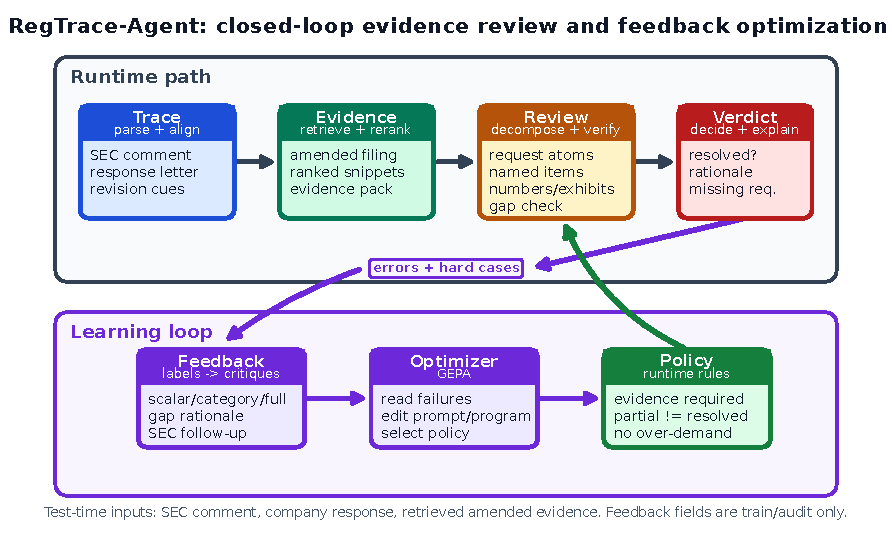
\includegraphics[width=\textwidth]{figures/regtrace_agent_framework.pdf}
\caption{\framework{} architecture. The runtime path parses a review trace, retrieves amended-filing evidence, checks request obligations, and emits a guarded verdict. The learning loop stores scalar, category, and natural-language feedback, lets GEPA revise the reviewer policy, and reinjects the learned policy into the obligation-review step. At test time the reviewer sees only the SEC comment, company response, and retrieved amended evidence.}
\label{fig:pipeline}
\end{figure*}

\subsection{SEC Instantiation}

Each SEC example contains three test-time fields: \texttt{sec\_comment}, \texttt{company\_response}, and \texttt{retrieved\_snippets} from amended filings. The output is binary. \texttt{resolved} means visible amended evidence covers the material request; \texttt{unresolved} means a named item, quantification, exhibit, document, legal analysis, accounting analysis, or other material requirement remains missing. The label is a visible-evidence judgment, not a legal determination or an inference from absence of later follow-up.

\subsection{SEC Trace Construction}

Figure~\ref{fig:pipeline} separates the runtime reviewer from the feedback-learning loop. In the SEC instantiation, we harvest \texttt{UPLOAD} and \texttt{CORRESP} materials from EDGAR, group staff comments and company responses into review threads, and select cases where the company claims a disclosure was added, revised, removed, or filed elsewhere. We identify amended filing candidates using filing metadata, amendment references, page and section cues, and response text. Candidate filings are drawn from a window of 10 days before to 60 days after the response date, with at most 8 candidate filings per row. A local lexical ranker retrieves top chunks, and an LLM reranker/adjudicator evaluates the top 3 snippets. From 589 revision-claim cases, 588 have candidate filings and snippets; 472 remain after requiring visible evidence that directly or partially addresses the SEC request. We then adjudicate whether visible evidence satisfies the request and construct labels plus feedback fields.

The retrieval component gives the agent evidence to inspect. The adjudication and feedback layer gives it something to learn from: what the reviewer asked for, what the company claimed to do, what the visible evidence supports, and what remains missing. These adjudication fields are not shown as ordinary test-time inputs. They are used for optimization feedback, audits, and analysis.

\subsection{Scale, Categories, and Splits}

\dataset{} contains 472 examples from 109 SEC review threads and 95 companies. The benchmark focuses on difficult revision-claim cases, and the label distribution is operationally realistic: 153 examples are \texttt{resolved}, and 319 are \texttt{unresolved}. Table~\ref{tab:data} summarizes the corpus and split regimes.

\begin{table}[t]
\centering
\small
\begin{tabular}{lr}
\toprule
\textbf{Quantity} & \textbf{Count} \\
\midrule
Examples & 472 \\
SEC review threads & 109 \\
Companies & 95 \\
Resolved / unresolved & 153 / 319 \\
Examples with verified follow-up & 236 \\
\midrule
Issue categories & 7 \\
Visible-evidence gap types & 8 \\
\bottomrule
\end{tabular}
\caption{Benchmark scale. Issue categories include other disclosure issues, risk factors, SPAC disclosure, revenue recognition, crypto, non-GAAP, and cybersecurity.}
\label{tab:data}
\end{table}

The corpus covers seven issue categories and eight visible-evidence gap types; Appendix~\ref{app:data} gives the full distribution. We use grouped, temporal, and topic-holdout regimes. The grouped split holds out entire review threads (229/104/139 train/dev/test). The temporal split trains on 2022--2023 and tests on 2024--2025 (264/64/144). The topic-holdout split tests transfer to held-out issue categories (279/68/125), including crypto and non-GAAP cases absent from training categories.

\subsection{From Labels to Feedback}

A standard benchmark would stop at binary labels. Our construction preserves the textual structure of each decision. For every example, adjudication records the material SEC request, the company action, evidence relevance, supporting evidence or resolution basis, visible unmet requirement, and a short rationale. This lets us compare increasingly rich optimization signals:
\begin{itemize}[leftmargin=*]
    \item scalar: correct or incorrect;
    \item category: correct/incorrect plus coarse issue or gap type;
    \item full: natural-language feedback describing the SEC request, company action, evidence coverage, and unmet requirement.
\end{itemize}
Full feedback can state that the evidence discusses combined revenue projections but fails to disclose entity-level operating costs, product pricing, gross margins, and forecast limitations. This is the reusable decision rule that scalar metrics discard.

\section{Methods}

\subsection{Prediction Setup}

The prediction model receives the SEC comment, company response, and raw retrieved amended-filing snippets. It returns a binary label and a short rationale. Explicit \texttt{resolved} is scored as resolved. \texttt{unresolved}, \texttt{partially\_resolved}, and other insufficient labels are normalized to unresolved. The rationale is required for inspection but not directly rewarded.

\subsection{Optimization Ladder}

We compare reviewer-training signals rather than evidence access. Baseline prompt is a handwritten reviewer instruction. MIPROv2 is scalar prompt optimization. GEPA-scalar uses reflective prompt optimization with correctness-only feedback. GEPA-category adds coarse category feedback. GEPA-full uses full natural-language adjudication feedback. We also include TF-IDF, a frozen sentence-encoder scoring head, a Jev typed decision gate, and an independent-feedback GEPA ablation for reviewer-facing robustness.

All methods receive the same evidence at test time, isolating the optimization signal rather than evidence access. The key comparison is whether natural-language feedback adds value beyond prompt search itself.

\subsection{Implementation Details}

All main prompt-optimization runs use \texttt{openai/gpt-4o-mini} as the frozen prediction model with temperature 0 and 500 output tokens. GEPA uses the same model as the reflection model with temperature 0.7 and 1500 reflection tokens, seed 17, \texttt{max\_metric\_calls}=150, reflection minibatch size 4, Pareto candidate selection, and 4 evaluation threads. MIPROv2 uses the same prediction and prompt models, 8 trials, 4 prompt candidates, and at most 4 labeled and 4 bootstrapped demonstrations. The frozen encoder scorer uses \texttt{all-MiniLM-L6-v2} with a logistic head over request, response, evidence, and request-evidence matching features. The Jev gate uses a \texttt{choice} question over \texttt{resolved}/\texttt{unresolved}. The evidence reranker/adjudicator also uses \texttt{gpt-4o-mini} at temperature 0. Model aliases rather than dated provider snapshots are recorded in the released artifacts.

\subsection{Optimization as Feedback-Conditioned Search}

We view each method as search over a prompt or prompt program $p$. Given an input $x$ and label $y$, the frozen LLM defines $\hat{y}_{p}(x)=f_{\theta}(x;p)$, and optimization seeks a prompt with high validation reward. The methods differ in what they observe after an error. Scalar optimization observes only correctness. Category feedback adds a coarse gap type. Full feedback adds a short critique describing the request, company action, visible evidence, and unmet requirement.

The intuition is information-theoretic. Let $C$ be the latent cause of failure, such as missing quantification or unsupported revision claim. Full feedback should help when it lowers uncertainty about $C$, because the optimizer can propose a more targeted semantic edit. This is not a general guarantee: a noisy or misaligned language channel can hurt. The hypothesis of \framework{} is that review traces are unusually well suited to language feedback because the failure causes are naturally written as reviewer critiques.

\subsection{What the Optimizer Sees}

During optimization, each candidate prompt is evaluated on development examples. When a prediction is incorrect, the metric returns feedback in one of three forms:
\begin{quote}
\small
\texttt{scalar: incorrect}\\
\texttt{category: incorrect; gap\_type=missing\_specific\_disclosure}\\
\texttt{full: incorrect. The SEC requested X. The company claimed Y. The visible evidence shows Z, but does not show required item W.}
\end{quote}
Full feedback summarizes the adjudicated relationship between the SEC request, response, and retrieved evidence for optimization examples only. It does not reveal hidden evidence at test time; any advantage must come from a better learned checklist for visible-evidence review.

\section{Experiments}

\subsection{Evidence Ablation}

We first test whether amended-filing evidence matters. Table~\ref{tab:evidence} evaluates a response-only condition, a raw-evidence condition, and an oracle evidence-summary condition on the grouped held-out test set.

\begin{table}[t]
\centering
\scriptsize
\setlength{\tabcolsep}{3pt}
\begin{tabular}{lrrrr}
\toprule
\textbf{Input} & \textbf{Acc.} & \textbf{Ma-F1} & \textbf{Res-F1} & \textbf{Unres-F1} \\
\midrule
Response only & 0.712 & 0.575 & 0.333 & 0.817 \\
+ raw snippets & 0.784 & 0.748 & 0.651 & 0.844 \\
+ oracle summary & 0.964 & 0.956 & 0.938 & 0.975 \\
\bottomrule
\end{tabular}
\caption{Evidence ablation. Adding raw amended-filing snippets raises macro-F1 by 17.3 points. The oracle summary is an upper bound, not a deployable baseline.}
\label{tab:evidence}
\end{table}

Response-only prompting cannot verify whether a revision claim is supported. Raw snippets nearly double resolved F1, while the oracle summary shows that much of the remaining difficulty is interpreting snippets against a specific request.

\subsection{Main Context-to-Feedback Results}

Table~\ref{tab:leaderboard} reports the main reviewer-training ladder on the frozen grouped split. All methods receive the same test-time context.

\begin{table*}[t]
\centering
\small
\begin{tabular}{lrrrrrr}
\toprule
\textbf{Method} & \textbf{Acc.} & \textbf{Macro-F1} & \textbf{Res-F1} & \textbf{Unres-F1} & \textbf{Unres-P} & \textbf{Unres-R} \\
\midrule
Majority unresolved & 0.691 & 0.409 & 0.000 & 0.817 & 0.691 & 1.000 \\
Baseline prompt & 0.424 & 0.402 & 0.518 & 0.286 & 1.000 & 0.167 \\
MIPROv2 & 0.655 & 0.652 & 0.619 & 0.684 & 0.929 & 0.542 \\
GEPA-scalar & 0.705 & 0.675 & 0.577 & 0.773 & 0.824 & 0.729 \\
GEPA-category & 0.597 & 0.595 & 0.562 & 0.627 & 0.870 & 0.490 \\
GEPA-full & \textbf{0.784} & \textbf{0.756} & \textbf{0.674} & \textbf{0.839} & 0.867 & \textbf{0.812} \\
\bottomrule
\end{tabular}
\caption{Frozen grouped-split leaderboard. GEPA-full gives the best macro-F1 and unresolved F1 under the same raw-evidence test-time context.}
\label{tab:leaderboard}
\end{table*}

The majority baseline has high accuracy because unresolved examples dominate, but zero resolved F1. The handwritten prompt is conservative: it has perfect unresolved precision but misses most gaps. MIPROv2 improves substantially, GEPA-scalar improves recall, and GEPA-category is too coarse in this run. GEPA-full is strongest overall, improving macro-F1 by 10.4 points over MIPROv2 and 8.1 points over GEPA-scalar. This shows that full feedback is not merely adding more text; it trains the reviewer to compare requested obligations against visible evidence.

Table~\ref{tab:robustness} addresses two alternate explanations and one deployment question. A TF-IDF logistic-regression classifier trained on the same raw evidence reaches only 0.523 macro-F1, so lexical supervision does not explain the GEPA-full gain. A frozen sentence encoder with a trained logistic scoring head reaches 0.667 macro-F1 without generation, and a Jev typed decision gate reaches 0.722, showing that \framework{} can support cheap triage scorers, but still trails the full feedback-trained reviewer. The guarded reviewer also improves over a monolithic prompt under both \texttt{gpt-4o-mini} and \texttt{gpt-5.4-mini}, suggesting that obligation-evidence structure matters across backbones. To test possible feedback leakage, we regenerate full textual feedback with an independent \texttt{gpt-5.4-mini} writer that sees only test-time fields plus the gold label, not the original adjudication rationales; GEPA with this feedback reaches 0.750 macro-F1, nearly matching the original 0.756.

\begin{table}[t]
\centering
\scriptsize
\setlength{\tabcolsep}{3pt}
\begin{tabular}{llr}
\toprule
\textbf{Check} & \textbf{Condition} & \textbf{Macro-F1} \\
\midrule
Lexical baseline & TF-IDF, response only & 0.523 \\
Lexical baseline & TF-IDF, raw snippets & 0.523 \\
Scoring head & Frozen encoder, raw snippets & 0.667 \\
Decision gate & Jev typed choice, raw snippets & 0.722 \\
Reviewer structure & 4o-mini monolithic / guarded & 0.638 / 0.808 \\
Reviewer structure & 5.4-mini monolithic / guarded & 0.612 / 0.732 \\
Feedback source & GEPA-full, original feedback & 0.756 \\
Feedback source & GEPA-full, independent feedback & 0.750 \\
Diagnostic upper bound & TF-IDF, oracle evidence summary & 0.858 \\
\bottomrule
\end{tabular}
\caption{Robustness checks. The raw-snippet TF-IDF baseline shows that lexical supervision does not explain the main result. Frozen encoder and Jev decision scorers are cheap non-generative triage components. Multi-LLM reviewer runs show that guarded obligation-evidence structure improves over monolithic prompting under two backbones. The independent-feedback ablation shows that GEPA-full does not depend on reusing the original adjudication rationales.}
\label{tab:robustness}
\end{table}

We also compute five-fold out-of-fold results over review-thread groups. Mean macro-F1 is 0.698 for GEPA-full, 0.647 for MIPROv2, 0.609 for GEPA-scalar, 0.545 for GEPA-category, and 0.446 for the handwritten baseline. The fold standard deviations are nontrivial (0.151 for GEPA-full and 0.121 for MIPROv2), so we treat the single grouped split as a headline comparison and the out-of-fold analysis as stability evidence rather than as a deterministic margin claim.

\subsection{Why Full Feedback Helps}

The advantage of GEPA-full is not simply risk aversion. Jev reaches very high unresolved recall (0.958) but lower resolved F1 (0.576), making it useful as a triage gate that flags likely unresolved responses. GEPA-full has lower unresolved recall but higher macro-F1, because it better balances skepticism with evidence sufficiency. It learns when a company revision claim is unsupported, but also when visible amended evidence already satisfies the SEC request.

The mechanism is visible in the feedback channel. Scalar feedback says only that a decision was wrong; category feedback names a coarse gap. Full feedback states what the SEC requested, what the company claimed, what the amended evidence showed, and what requirement remained unmet. This gives the optimizer a reusable review trace rather than a bare reward. The resulting prompt evolution shifts from generic caution to obligation-level comparison: identify material SEC request elements, inspect amended evidence for named disclosures, quantification, exhibits, and legal or accounting analysis, and distinguish partial disclosure from resolution.

The trade-off is cost and calibration. GEPA-full requires adjudicated natural-language feedback and offline optimization, so it is not the cheapest runtime gate. It can also become over-skeptical when evidence substantially satisfies a request but does not present the answer in the exact form the prompt expects. We therefore view Jev and frozen encoders as high-throughput first-pass gates, and GEPA-full as the deeper reviewer for difficult or high-impact cases.

\subsection{Reviewer-Structure Ablation}

The optimization ladder tests feedback richness. We also ask whether reviewer structure matters. Table~\ref{tab:guarded} compares a monolithic judgment, an obligation-guided judgment, and a guarded verifier that requires every material obligation to be visibly satisfied, with GEPA-full as the optimized-prompt reference.

\begin{table}[t]
\centering
\scriptsize
\setlength{\tabcolsep}{4pt}
\begin{tabular}{lrrr}
\toprule
\textbf{Reviewer} & \textbf{Macro-F1} & \textbf{Res-F1} & \textbf{Unres-F1} \\
\midrule
Monolithic reviewer & 0.645 & 0.614 & 0.676 \\
Obligation-guided reviewer & 0.619 & 0.613 & 0.624 \\
GEPA-full optimized prompt & 0.756 & 0.674 & 0.839 \\
RegTrace guarded verifier & \textbf{0.801} & \textbf{0.727} & \textbf{0.874} \\
\bottomrule
\end{tabular}
\caption{Reviewer-structure ablation. The guarded verifier is a policy-distillation prototype derived from the obligation-evidence policy exposed by GEPA-full prompt evolution.}
\label{tab:guarded}
\end{table}

Simply listing obligations is not enough; the gain comes from the guard that requires visible support for each material request. We report this as a policy-distillation prototype rather than the primary optimizer comparison, since it adds human-designed structure after prompt-evolution analysis.

\subsection{Feedback Component Ablation}

Table~\ref{tab:feedback} holds test-time input fixed and changes only optimization-time feedback.

\begin{table*}[t]
\centering
\small
\begin{tabular}{lrrrrrr}
\toprule
\textbf{Feedback} & \textbf{Acc.} & \textbf{Macro-F1} & \textbf{Res-F1} & \textbf{Unres-F1} & \textbf{Unres-P} & \textbf{Unres-R} \\
\midrule
Full feedback & 0.784 & \textbf{0.756} & \textbf{0.674} & 0.839 & 0.867 & 0.812 \\
No evidence rationale & 0.712 & 0.682 & 0.583 & 0.780 & 0.826 & 0.740 \\
No unmet requirement & 0.741 & 0.708 & 0.609 & 0.806 & 0.833 & 0.781 \\
Request + action only & 0.784 & 0.724 & 0.595 & \textbf{0.853} & 0.806 & \textbf{0.906} \\
\bottomrule
\end{tabular}
\caption{Feedback component ablation. Request-action feedback induces aggressive unresolved detection, while full feedback gives the best macro-F1 by calibrating skepticism with evidence rationales.}
\label{tab:feedback}
\end{table*}

Request-action-only feedback induces aggressive skepticism and the highest unresolved recall, but sacrifices resolved F1. Full feedback teaches both sides of the boundary: unmet requirements for unresolved cases and supporting evidence for resolved cases.

\subsection{Temporal and Topic Generalization}

Table~\ref{tab:gen} shows that the optimized prompt transfers beyond the grouped split. In the temporal setting, GEPA-full trains/tunes on 2022--2023 and tests on 2024--2025 material. In the topic setting, test examples include crypto and non-GAAP cases absent from training issue categories.

\begin{table*}[t]
\centering
\small
\begin{tabular}{llrrrr}
\toprule
\textbf{Split} & \textbf{Method} & \textbf{Acc.} & \textbf{Macro-F1} & \textbf{Unres-F1} & \textbf{Unres-R} \\
\midrule
\multirow{4}{*}{Time} 
& Baseline & 0.451 & 0.434 & 0.336 & 0.206 \\
& MIPROv2 & 0.521 & 0.519 & 0.489 & 0.340 \\
& GEPA-scalar & 0.653 & 0.650 & 0.679 & 0.546 \\
& GEPA-full & \textbf{0.826} & \textbf{0.791} & \textbf{0.877} & \textbf{0.918} \\
\midrule
\multirow{4}{*}{Topic}
& Baseline & 0.440 & 0.440 & 0.426 & 0.274 \\
& MIPROv2 & 0.576 & 0.565 & 0.635 & 0.484 \\
& GEPA-scalar & 0.528 & 0.524 & 0.569 & 0.411 \\
& GEPA-full & \textbf{0.784} & \textbf{0.734} & \textbf{0.849} & \textbf{0.800} \\
\bottomrule
\end{tabular}
\caption{Temporal and topic-holdout generalization. GEPA-full transfers substantially better than scalar optimization.}
\label{tab:gen}
\end{table*}

The topic-holdout result argues against a curated-topic explanation. Per-topic breakdowns show GEPA-full improves over MIPROv2 on crypto, non-GAAP, revenue recognition, risk factors, and broad other-disclosure cases, with largest gains in revenue recognition and non-GAAP.

\section{External SEC Follow-Up Corroboration}

Visible-evidence labels come from an adjudication pipeline, so we test whether they align with later regulator behavior. Verified same-topic next-round SEC follow-up is not the primary label, but it is a useful corroboration signal because it can restate or narrow an unresolved gap.

We additionally audit 60 examples with an independent LLM auditor that receives the SEC comment, company response, and visible amended evidence but not the original label rationale. The audit agrees with the benchmark label in 49 of 60 cases, with mean confidence 0.897. We report this as an audit of visible-evidence label consistency, not as expert legal/accounting validation.

\begin{table}[t]
\centering
\scriptsize
\setlength{\tabcolsep}{2pt}
\begin{tabular}{lrrr}
\toprule
\textbf{Group} & \textbf{N} & \textbf{D/P} & \textbf{Rate} \\
\midrule
Unres. + f/u & 160 & 109 & 68.1\% \\
Res. + f/u & 76 & 7 & 9.2\% \\
\bottomrule
\end{tabular}
\caption{Real follow-up corroboration. Later same-topic SEC comments directly or partially corroborate unresolved visible-evidence labels far more often than resolved labels.}
\label{tab:followup}
\end{table}

Among 236 examples with verified follow-up, unresolved cases are corroborated at 68.1\%, while resolved cases are corroborated at only 9.2\% (Table~\ref{tab:followup}). Follow-up availability itself is balanced across labels (49.7\% for resolved and 50.2\% for unresolved; Fisher exact $p=1.0$), so this is not merely an availability artifact.

Following reviewer-style paired analysis, we also treat later follow-up as a noisy external reference on a clean 220-example subset. The benchmark label reaches 0.756 macro-F1 against this signal, compared with 0.590 for five-fold out-of-fold GEPA-full predictions and 0.460 for the handwritten baseline. We therefore use follow-up primarily as label-validity evidence, not as proof that every GEPA-full win is separately corroborated beyond the unresolved base rate.

In one expense-disclosure case, the SEC asked for material components and trend discussion. The company claimed a revision, but retrieved evidence showed only a line item and totals; GEPA-full predicted \texttt{unresolved}, and the next-round SEC follow-up again requested the component breakout. SPAC transaction-background cases show the same pattern for missing negotiation details.

\section{Prompt Evolution and Case Studies}

\subsection{Prompt Evolution}

Prompt evolution shows that GEPA-full does not merely make the prompt longer. It turns adjudication feedback into a compact regulatory reading policy. The seed prompt is a single sentence; the final GEPA-full run saves optimized candidates of 349 and 397 words (Appendix~\ref{app:prompts}).

\begin{table}[t]
\centering
\scriptsize
\setlength{\tabcolsep}{3pt}
\begin{tabular}{lrrrr}
\toprule
\textbf{Method} & \textbf{Claim} & \textbf{Evidence} & \textbf{Request} & \textbf{Missing} \\
 & \textbf{insuff.} & \textbf{required} & \textbf{match} & \textbf{items} \\
\midrule
GEPA-full & 2/2 & 2/2 & 2/2 & 2/2 \\
GEPA-scalar & 2/2 & 2/2 & 0/2 & 0/2 \\
GEPA-category & 2/2 & 2/2 & 0/2 & 0/2 \\
Req.+action only & 2/2 & 2/2 & 2/2 & 2/2 \\
\bottomrule
\end{tabular}
\caption{Rule presence in optimized prompt candidates. Full feedback more consistently induces named-request matching and missing-item reasoning.}
\label{tab:prompt}
\end{table}

Scalar and category feedback learn general caution: do not trust a revision claim unless evidence supports it. Full feedback more consistently learns named-request matching and missing-item reasoning (Table~\ref{tab:prompt}), shifting from generic skepticism to obligation-level comparison: SEC request $\rightarrow$ company action $\rightarrow$ visible evidence $\rightarrow$ remaining gap.

\subsection{Method-Disagreement Cases}

The strongest GEPA-full wins involve concrete request-evidence mismatches. In a financial-projections case, the SEC requested individual-company forecast information and material assumptions; the amended evidence showed only combined revenue projections. GEPA-full marked it unresolved because the requested assumption set was still absent.

In a crypto terminology case, the amended evidence defined stablecoins but did not explain the SEC's requested contrast with unstable cryptocurrency. Baseline, MIPROv2, GEPA-scalar, and GEPA-category predicted \texttt{resolved}; GEPA-full predicted \texttt{unresolved}. In a PIPE financing case, MIPROv2 treated the presence of price terms as sufficient; GEPA-full required equivalent price-per-share disclosure for each agreement, a gap later echoed in SEC follow-up.

GEPA-full also has informative errors. In one ownership-percentage case, retrieved evidence contained redemption-scenario calculations and the benchmark label was \texttt{resolved}. GEPA-full predicted \texttt{unresolved} because it wanted a more explicit cover-page presentation. This reveals the main calibration risk: full-feedback prompts learn useful skepticism but can over-require exact presentation. Appendix~\ref{app:cases} lists additional cases.

\section{Discussion}

The main result is not simply that one optimizer beats another. \framework{} turns a recurring compliance pattern into an offline feedback-learning system: collect the trace, retrieve the revised artifact, check obligations against visible evidence, issue a guarded verdict, and recycle adjudicated failures as feedback. The learned reviewer can be used directly, distilled into a guarded verifier, or converted into lightweight scoring heads for high-throughput triage. The output is a traceable unresolved-gap rationale, not only a binary label.

Language feedback helps because it preserves decision structure. A scalar signal says only that a verdict failed; full feedback says which named request, company action, amended snippet, and remaining obligation were mismatched. The optimized prompt therefore becomes an interpretable policy: extract material requests, distrust unsupported revision claims, inspect evidence for named items, avoid over-requiring, and distinguish partial disclosure from resolution.

SEC correspondence is the public setting where we can observe request, response, revised filing, and later reviewer behavior, but the trace structure is broader. Audit remediation, regulatory reporting, lending-document stipulations, data-quality exceptions, and internal compliance monitoring also contain request-response-evidence loops. The transferable claim is that such traces can support retrieval, obligation checking, adjudication feedback, optimized reviewing, and hard-case mining; the limitation is that high-recall language-feedback policies can become over-skeptical.

\section{Conclusion}

We introduced \framework{}, a context-to-feedback framework for evidence-grounded response review, and instantiated it as \dataset{} using public SEC traces. Across grouped, temporal, and topic-holdout evaluations, full natural-language feedback yields the strongest reviewer. Evidence ablations, prompt evolution, and SEC follow-up corroboration suggest that financial NLP benchmarks can move from static labels toward feedback-rich review systems that preserve the reasons behind expert decisions.

\section*{Limitations and Data Statement}

This study is conditioned on visible retrieved evidence, so missed snippets can affect labels. The benchmark is LLM-adjudicated, with independent audit and external follow-up corroboration but without a full expert legal/accounting audit. A full independent \texttt{gpt-5.4-mini} audit over all 472 examples, using only test-time fields, reaches 0.731 agreement accuracy and 0.715 macro-F1 against the released labels. Same-topic SEC follow-up is a noisy behavioral signal, not ground truth. We frame labels as visible-evidence judgments rather than legal determinations. An anonymized release will be provided at \url{https://anonymous.4open.science/r/regtrace-sec-XXXX/}; it includes benchmark JSONL, splits, accession identifiers, retrieval metadata, snippets, labels, feedback fields, prompts, outputs, and analysis scripts.

\clearpage
\bibliography{references}

\appendix

\section{Full Optimized Prompts}
\label{app:prompts}

The main paper quotes short excerpts from optimized prompts. Below are the full GEPA-full optimized candidates exposed by the final grouped-split run. The seed prompt was: ``Classify whether a company resolved an SEC comment using the visible evidence.''

\subsection{GEPA-full Optimized Candidate 1}

\begin{quote}\small
You are tasked with classifying whether a company has resolved a comment from the SEC based on the provided evidence. Follow these instructions carefully:

1. Input Format: You will receive three types of inputs: \texttt{sec\_comment}, \texttt{company\_response}, and \texttt{amended\_evidence}.

2. Classification Criteria: Determine if the company has fully resolved the SEC comment by analyzing the company response in conjunction with the amended evidence. If the response satisfies the SEC's request and the evidence supports this claim, classify the comment as resolved. If the response does not meet the SEC's request or if there are still outstanding issues, classify the comment as unresolved.

3. Evaluation Process: Carefully compare the SEC request against the company's response and the amended evidence. Look for specific items or information requested by the SEC, quantification or detailed analysis that meets SEC requirements, references to regulatory guidance or previous decisions, and clear explanations of how the company adjusted disclosures or practices. Take note of visible unmet requirements, partial fixes, or lack of supporting documentation in the amended evidence.

4. Output Format: Include a reasoning section, a label indicating resolved or unresolved, and a concise reason.

5. Feedback Incorporation: Be vigilant about claims made by the company; ensure that amended evidence corroborates these claims. Identify instances where the response may partially address SEC concerns but still falls short of complete compliance.
\end{quote}

\subsection{GEPA-full Optimized Candidate 2}

\begin{quote}\small
You are tasked with classifying whether a company has resolved a comment issued by the SEC based on provided evidence. Follow these specific instructions for the task:

1. Input Format: You will receive \texttt{sec\_comment}, \texttt{company\_response}, and \texttt{amended\_evidence}. The SEC comment is the original request for clarification or additional information. The company response indicates what changes were made or explanations provided. The amended evidence contains snippets from the amended filing or other documents that support the response.

2. Classification Criteria: Determine whether the company's response and amended evidence adequately address the SEC's concerns as outlined in the original comment. A response is resolved if it fully satisfies the requirements of the SEC comment, including clear explanations, specific details, and quantifications when necessary. A response is unresolved if there are still gaps or missing elements in the company's explanation or if amended evidence does not address all parts of the SEC comment.

3. Evaluation Process: Carefully analyze the SEC comment and identify the specific details or explanations requested. Review the company response to see if the company acknowledged the comment and provided a meaningful response. Examine amended-evidence snippets to confirm that they support the company's claims and cover all requested aspects of the SEC comment. Look for direct references in the amended evidence that address the SEC's specific requests, such as ownership structures, accounting adjustments, or enforcement risks.

4. Labeling: If the company has fully addressed the SEC's concerns with adequate evidence, label the response resolved. If there are omissions or inadequacies in addressing SEC requests, label it unresolved.

5. Justification: Provide clear and concise reasoning that cites specific elements from the SEC comment, company response, and amended evidence. Highlight specific unmet requirements or gaps in the evidence that contribute to an unresolved classification.

6. Feedback Incorporation: Pay attention to feedback from previous examples to identify common pitfalls, such as failing to compare the SEC request against the evidence adequately or missing key elements in the response.
\end{quote}

\section{Additional Dataset Details}
\label{app:data}

The most common issue categories are other disclosure issues (183), risk factors (91), SPAC disclosure (78), revenue recognition (75), crypto (28), non-GAAP (16), and cybersecurity (1). The most common gap types are resolved visible evidence (153), missing specific disclosure (140), missing quantification (59), resolved-but-regulator-requested-more-detail (38), missing exhibit or document (29), incomplete accounting analysis (25), incomplete legal or regulatory analysis (25), and other visible evidence gap (3).

\section{Additional Qualitative Cases}
\label{app:cases}

The qualitative appendix used during analysis includes full SEC comments, company responses, amended evidence snippets, method predictions, GEPA-full rationales, and later SEC follow-up text for selected cases. These include stablecoin terminology, financial forecast assumptions, PIPE price-per-share disclosure, Item 404 related-party disclosure, expense breakout and trend discussion, and SPAC transaction-background disclosure.

\end{document}
